\begin{frame}[fragile]
  \frametitle{Machine characteristics}
  \begin{columns}
    \begin{column}{0.55\textwidth}
      \begin{itemize}
      \item Unprecedented levels of available concurrency
        \begin{itemize}
        \item IBM BG/Q
          \begin{itemize}
          \item `Sequoia': 1,572,864 cores
          \item `Mira': 786,432 cores
          \end{itemize}
        \item Cray
          \begin{itemize}
          \item XE6 `Bluewaters`: $>$ 380,000 cores
          \item XK6 `Titan': 299,008 cores
          \end{itemize}
        \item K Supercomputer: 705,024 cores
        \end{itemize}
      \end{itemize}
    \end{column}
    \begin{column}{0.45\textwidth}
      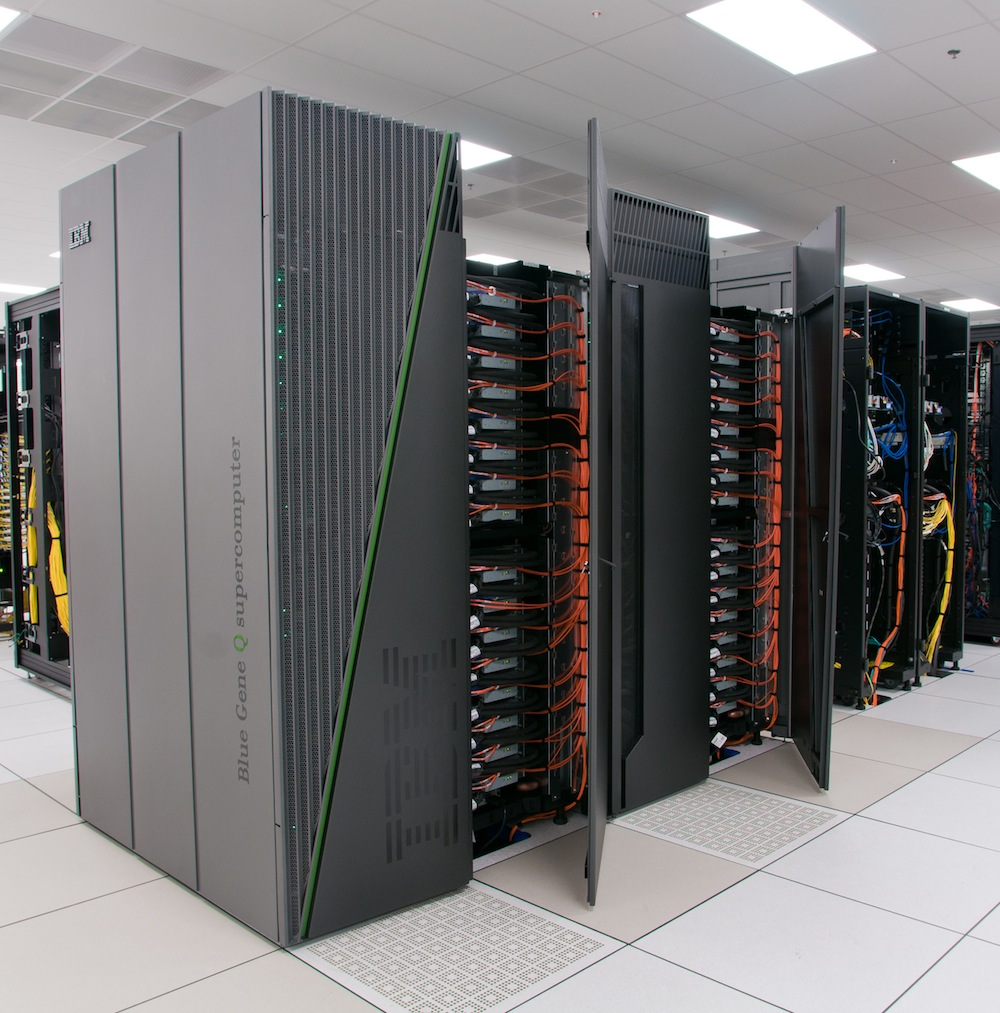
\includegraphics[width=1\textwidth]{figures/mira.jpg}
    \end{column}
  \end{columns}
\end{frame}

\begin{frame}[fragile]
  \frametitle{Machine characteristics}
  \begin{itemize}
  \item Longer data movement latencies (memory and network)
  \item Architecture heterogeneity
  \item Extracting performance on tighter power / energy budget
  \item Hardware component failures / faults
  \end{itemize}
\end{frame}

\begin{frame}[fragile]
  \frametitle{Application characteristics}
  \begin{itemize}
  \item Complex physics in multiple, interacting modules
  \item Adaptive, spatial and temporal resolutions
  \item Need for faster solutions (not just larger problems)
  \end{itemize}
\end{frame}

\begin{frame}[fragile]
  \frametitle{MPI Stencil Pseudo-code}
  \begin{itemize}
  \item 
  \end{itemize}
\end{frame}